\documentclass[11pt, a4paper, oneside]{book}
\usepackage[margin=1in]{geometry}
\usepackage{amsfonts, amsmath, amssymb, bm, extarrows}
\usepackage[none]{hyphenat}%prevent hyphenated words
\usepackage{fancyhdr}
\usepackage{graphicx, float}

\allowdisplaybreaks%允许公式换页
\def\D{\partial}

\setcounter{tocdepth}{1}

\numberwithin{equation}{section}%mark: niubi
\pagestyle{fancy}
\fancyhead{}
\fancyhead[L]{\slshape \MakeUppercase{Physics I}}
\fancyhead[R]{\slshape HYJ}
\fancyfoot[C]{\thepage}

\begin{document}
	
	\begin{titlepage}
		\begin{center}
			\Large{\textbf{University Physics I}}\\
			\vfill%vertical fill
			\line(1,0){400}\\[1mm]
			\huge{\textsc{Classic Mechanics: Review}}\\[3mm]
			\Large{- \textit{``I now demonstrate the frame of the system of the world.''} -}\\[1mm]
			\line(1,0){400}\\
			\vfill
			By HYJ \\
			\today
		\end{center}
	\end{titlepage}

\tableofcontents
\thispagestyle{empty}





%----------------------------------

%----------------------------------
\chapter{Highlights}

To organize and memorize.
%----------------------------------
%----------------------------------
\section{Introduction}

An introduction to the course.\\ 
``All equations of vectors can be written in the form of its components.''\\

\textbf{Contents}
\begin{itemize}
	\item Vectors and its components
	\item Coordinates
\end{itemize}

\textbf{Highlights}
\begin{enumerate}
	\item Polar coordinates\\
	Components calculation:\\
	$\left\{\begin{aligned}
	\frac{d\bm{e}_\rho}{dt} &= \dot{\phi}\bm{e}_\phi\\
	\frac{d\bm{e}_\phi}{dt} &= -\dot{\phi}\bm{e}_\rho
	\end{aligned}\right.$\\
	$\left\{\begin{aligned}
	\bm{\rho} &= \rho \bm{e}_\rho\\
	\dot{\bm{\rho}} &= \dot{\rho} \bm{e}_\rho + \rho \dot{\phi} \bm{e}_\phi\\
	\ddot{\bm{\rho}} &= (\ddot{\rho} - \rho\dot{\phi}^2 )\bm{e}_\rho + (2\dot{\rho}\dot{\phi} + \rho\ddot{\phi})\bm{e}_\phi
	\end{aligned}\right.$\\
	$ \bm{e}_\rho = 0 $ in circular motion.

	\item Spherical polar coordinates\\
	$(\bm{e}_r, \bm{e}_\theta, \bm{e}_\phi)$~~~~~~~~$\bm{A} = A_r\bm{e}_r + A_\theta\bm{e}_\theta + A_\phi\bm{e}_\phi $\\
	Components calculation:\\
	$\left\{
	\begin{aligned}
	\bm{e}_r &= \cos\theta\bm{k} + \sin\theta(\cos\phi\bm{i} + \sin\phi\bm{j})\\
	\bm{e}_\theta &= -\sin\theta\bm{k} + \cos\theta(\cos\phi\bm{i} + \sin\phi\bm{j})\\
	\bm{e}_\phi &= -\sin\phi\bm{i} + \cos\phi\bm{j}
	\end{aligned}
	\right.$\\
\end{enumerate}

%----------------------------------
%----------------------------------
\section{Kinematics}

An introduction to classical mechanics. \\

\textbf{Contents}
\begin{itemize}
	\item Translational motion
	\item Rotational motion
		\begin{itemize}
			\item Orbiting: Coriolis acceleration*\footnote{ * means difficult and need extra attention. Not optional.}
		\item Oscillation: Simple pendulum
		\end{itemize}
	\item Oscillation
		\begin{itemize}
			\item *Phase space
		\end{itemize}
	\item Galilean transformation: $\dot{\bm{r}}' = \dot{\bm{r}} - \bm{u}$
\end{itemize}

\textbf{Highlights}
\begin{enumerate}
	\item Coriolis acceleration: $\bm{a}_S = \bm{a}_{S^{'}} + 2 (\bm{\omega} \times \bm{v}_{S^{'}}) + \bm{\omega} \times (\bm{\omega}\times \bm{r})$
\end{enumerate}

%----------------------------------
%----------------------------------
\section{Particle Dynamics}

Basic analytical tools and methods used in classical mechanics.\\
``Nature and nature's laws lay hid in night;
God said `let Newton be' and all was light.''\\

\textbf{Contents}
\begin{itemize}
	\item Newton's second \& third law
		\subitem Non-inertial frame \& inertial force
	\item Momentum \& angular momentum
	\item Mechanical work \& energy 
\end{itemize}

\textbf{Highlights}
\begin{enumerate}
	\item Newton's second law\\
	$\bm{F} = m\bm{a}$
	\item Non-inertial frame \& inertial force\\
	$ (\bm{F} + \bm{F}_{in} ) = m\bm{a}' $~~~~~~~~$ \bm{F}_{in} \equiv - m\dot{\bm{u}} $~~~~~~~~$\bm{u}$: speed of $S'$ in $S$.
	
	\item Momentum: \textbf{Integral of force over time.}\\
	$ \bm{p} = m\bm{v} $\\
	\large{$ \dfrac{d\bm{p}}{dt} = \bm{F} $}
	
	impulse-momentum relation: \\
	$ \bm{p}_f - \bm{p}_i = \bar{\bm{F}}\left(t_f - t_i\right) $
	
	\item Angular momentum\\
	$ \bm{L} = \bm{r} \times \bm{p} = I\omega$\\
	\large{$ \dfrac{d\bm{L}}{dt} = \bm{M} = \bm{r} \times \bm{F} = I \alpha$}
	
	\item Work \& energy: \textbf{Integral of force over space.}\\
	$ -\Delta U = W = \int \bm{F}d\bm{r} = \Delta T$\\
	\large{$ \dfrac{dW}{dr} = F $}
	
	$ E = U + T = Const. $

\end{enumerate}

%----------------------------------
%----------------------------------
\section{Gravitation}
Study of gravitational force.\\
``Mensus eram coelos, nunc terrae metior umbras. Mens coelestis erat, corporis umbra iacet.''\\

\textbf{Contents}
\begin{itemize}
	\item 3 (most) useful tools
		\begin{itemize}
			\item law of gravitation
			\item gravitational potential energy\\
			\item conservation of angular momentum
		\end{itemize}
	\item 3 Gravitational phenomenon
		\begin{itemize}
			\item gravitational mass
			\item gravitational redshift
			\item gravitational collapse
			\item tidal force*
		\end{itemize}
	\item 3 Kepler problems*

\end{itemize}

\textbf{Highlights}
\begin{enumerate}
	\item The law of gravitation: $\bm{F} = -G\dfrac{m'm}{r^3}\bm{r}$
	\item Gravitational potential energy: first integral over $ r $ of the equation above.\\
	$\left\{\begin{aligned}
	 U &= -G\dfrac{m'm}{r}, \infty \rightarrow r\\
	 U &= -G\dfrac{m'm}{R+h} + G\dfrac{m'm}{R} = mgh\dfrac{1}{1 + h/R}, R \rightarrow R + h
	\end{aligned}\right.$
	\item Gravitational self-energy (of a uniform sphere):
	$U_s = -G\dfrac{3m^2}{5R}$
	\item Black Hole: $r_g = \dfrac{2GM}{c^2}$
	\item Gravitational redshift:
	$ hd\nu = mgdz = \dfrac{h\nu}{c^2}gdz $ (Energy)
	
	$v_0 = v_e \exp\left\{-\dfrac{g}{c^2}H\right\} \sim v_e\left(1 - \dfrac{g}{c^2}H\right)$
	
	$v_0 = v_e \exp\left\{-\dfrac{Gm'}{R_c^2}H\right\} \sim v_e\left(1 - \dfrac{Gm'}{R_c^2}H\right)$
	\item Kepler problems
	\begin{enumerate}
		\item the problem of orbit*
			\subitem Effective Potential: $E \equiv \dfrac{1}{2}\mu \dot{r}^2 + U_{\text{eff}}(r) = \dfrac{1}{2}\mu \dot{r}^2 + \dfrac{L^2}{2\mu r^2} + U(r) \left(= \dfrac{1}{2}\mu \dot{r}^2 + \dfrac{L^2}{2\mu r^2} - \dfrac{k}{r}\right)$
		\item the problem of area: $\dfrac{dA}{dt} = \dfrac{d(L/2\mu)}{dt} = 0$
		\item the problem of period: $T = \dfrac{\pi ab}{L/2\mu} = \dfrac{2\mu\pi}{L}a^{3/2}\sqrt{p} = 2\pi a^{3/2}\sqrt{\dfrac{1}{G(m' + m)}} $
	\end{enumerate}
	\item Gravitational field \& potential: $\bm{g}_f \equiv -\bigtriangledown V$~~~~$V = -G\dfrac{m'}{r} + C$
	\item Tidal force: 
	$\left\{\begin{aligned}
	\bm{g}_f &= \dfrac{Gm}{r^2}\bm{k} + g_r\bm{e}_r + g_\theta\bm{e}_\theta\\
	g_r &= \dfrac{Gm}{a^2}\dfrac{r}{a}(3\cos^2\theta - 1)\\
	g_\theta &= -G\dfrac{m}{a^2}\dfrac{r}{a}(3\cos\theta\sin\theta)	 
	\end{aligned}\right.$
	\item Tidal Disruption: $ \rho\Delta m \left(\dfrac{2Gm'}{a^3} + \omega^2 - \dfrac{Gm}{r^3}\right) > 0 $

\end{enumerate}

%-------------------------------------
%-------------------------------------

\section{Dynamics of Many-Particle System}

Study interaction between particles and the system as a whole.\\

\textbf{Contents}
	\begin{itemize}
		\item COM
		\item Variable mass \& Collisions
		\item Fluid motion
	\end{itemize}

\textbf{Highlights}
	\begin{enumerate}
		\item The center of mass: $\displaystyle{\bm{r}_C = \dfrac{\sum^N_i (m_i \bm{r}_i)}{m_C} = \dfrac{1}{m_C}\int \rho \bm{r}d\tau}$
		\item COM system: \\
		$p = 0$\\
		$\dfrac{d}{dt}\bm{L} = \bm{M}$\\
		$\displaystyle{T = T_C + \sum^N_i T'_i}$\\
		$\displaystyle{U = \sum^N_i U_i + \dfrac{1}{2}\sum^N_{\substack{i, j \\ i \neq j}} U_{ij} = \sum^N_i U_i + \sum^N_{\substack{i, j \\ i > j}} U_{ij}}$
		\item Classical collision: \\
		$\left\{\begin{aligned}
		v_1' = \dfrac{m_1 - m_2}{m_1 + m_2}v_1\\
		v_2' = \dfrac{2m_1}{m_1+m_2}v_1
		\end{aligned}\right.$
		\item Coefficient of restitution: $e = \dfrac{v_2' - v_1'}{v_1 - v_2} $, $ 0 \leq e < 1 $
		\item Motion of fluid\\
		$Av = \text{Const.}$\\
		Bernoulli equation (in the reference frame in which the flow is steady):\\
		$p + \dfrac{1}{2}\rho v^2 + \rho g h = \text{Const.}$
	\end{enumerate}

%-------------------------------------
%-------------------------------------

\section{Dynamics of a Rigid Body}

\textbf{Contents}
	\begin{itemize}
	\item Rotation inertia
	\item Dynamics of rotation
	\item Precession
	\item Equilibrium \& stability
	\end{itemize}

\textbf{Highlights}
	\begin{enumerate}
		\item Rotation inertia: $\displaystyle{I \equiv \int\rho^2\,dm}$\\
			\begin{enumerate}
				\item A ring: $I_\perp = mR^2$, $I_\parallel = \dfrac{1}{2}mR^2$
				\item A sphere/spherical shell: $I = \dfrac{2}{5}mR^2$
				\item A hollow cylinder: $I = \dfrac{1}{2}m(R^2_1 + R^2_2)$
				\item A cylinder or gyration: $I = \dfrac{1}{2}mR^2$
				\item A stick: $I_{\text{mid}} = \dfrac{1}{12}ml^2$, $I_{\text{side}} = \dfrac{1}{3}ml^2$
				\item A thin plate: $I_{z} = \dfrac{1}{6}ml^2$, $I_{xy} = \dfrac{1}{12}ml^2$
			\end{enumerate}
		\item Parallel axis theorem: $I = I_C + md^2$
		\item Perpendicular axis theorem: $I = I_x + I_y$
		\item Dynamics of rotation:\\
			$M = I\alpha$
			
			$\alpha \equiv \dfrac{d}{dt}\omega$
		\item Rotation kinetic energy: 
			$\dfrac{1}{2}m_Cv_C^2 + \dfrac{1}{2}I\omega^2 + U = \text{Const.}$ 
		\item Work: 
			$dW = Md\phi$
		\item Power:
			$P = \bm{M}\cdot \bm{\omega}$
		\item Precession(angular velocity):
			$ \Omega = \dfrac{rmg}{I\omega} $
		\item Equilibrium \& stability:\\
			$ U' = 0 \text{ equilibrium,} $\\
			$ U'' \left\{\begin{aligned}
			&> 0 \text{ stable,} \\
			&= 0 \text{ neutral,} \\
			&< 0 \text{ unstable.}
			\end{aligned}\right.$
	\end{enumerate}


\section{Oscillations}

\textbf{Contents}
	\begin{itemize}
		\item SHO
		\item Coupled Oscillation
		\item Damped Oscillation
		\item Forced Oscillation
	\end{itemize}

\begin{enumerate}
	\item SHO: $A$, $\omega_0$, $\phi$
\begin{flalign*}
	&m\ddot{x} + kx = 0&\\
	&\ddot{x} + \omega_0^2x = 0&\\
	&\left\{\begin{aligned}
	x &= A\cos(\omega t + \phi)\\
	A &= \left(x_0^2 + \dfrac{\dot{x}^2}{\omega_0^2}\right)^{1/2}\\
	\phi &= \arctan \left(-\dfrac{\dot{x}_0}{\omega x_0}\right)\\
	\omega_0 &= \sqrt{\dfrac{k}{m}}
	\end{aligned}\right.&\\
	&E = \dfrac{1}{2}m\dot{x} + \dfrac{1}{2}m\omega_0^2x^2=\text{Const.}&\\
\end{flalign*}
	\item Coupled Oscillation: Normal Frequency: $\omega_1$, $\omega_2$\\
	2 Cases:
\begin{flalign*}
	&\omega_1 = \sqrt{k_0/m}&\\
	&\omega_2 = \sqrt{(k_0 + 2k)/m}&
\end{flalign*}
	\item Damped Oscillation: $Q$
\begin{flalign*}
	&m\ddot{x} + kx + \eta\dot{x} = 0&\\
	&\ddot{x} + \omega_0^2x + 2\gamma\dot{x} = 0&\\
	&\gamma = \dfrac{\eta}{2m},\quad\omega_0 = \sqrt{\dfrac{k}{m}}&
\end{flalign*}
	\begin{enumerate}
		\item Light damping: $\gamma < \omega_0$\\
			$\left\{\begin{aligned}
			&x = Ae^{-\gamma t}\cos(\omega t + \phi)\\
			&\omega^2 = \omega_0^2 - \gamma^2
			\end{aligned}\right.$
		\item Critical damping*: $\gamma = \omega_0$\\
			$x = (a + bt)e^{-\gamma t}$
		\item Over/Heavy damping*: $\gamma > \omega_0$\\
			$x = a^{-\gamma t}\left[\cos(\beta t)+b\sin(\beta t)\right],\quad\beta = \sqrt{\gamma^2 - \omega_0^2}$
	\end{enumerate}
Energy flow in a period (\textit{Quality Factor}):
\begin{flalign*}
	&-\dfrac{1}{\langle E \rangle}\dfrac{d\langle E \rangle}{dt}T=2\gamma\dfrac{2\pi}{\omega} \equiv \dfrac{2\pi}{Q},\quad Q \equiv \dfrac{\omega}{2\gamma} = \dfrac{m\omega}{\eta}&
\end{flalign*}
	\item Forced Oscillation Under Friction
	Equation of Motion
\begin{flalign*}
	&\ddot{x} + \omega_0^2x + 2\gamma\dot{x} = \dfrac{F_0}{m}\cos\omega t&\\
	&x = \dfrac{F_0/m}{\sqrt{(\omega^2 - \omega_0^2)^2 + 4\gamma^2\omega^2}}\cos\left(\omega t-\dfrac{\pi}{2} + \arctan\dfrac{\omega_0^2 - \omega^2}{2\gamma\omega}\right)&\\
	&A = \dfrac{F_0}{k},\quad \omega = 0&
\end{flalign*}
	\begin{enumerate}
		\item Displacement resonance: at $\omega^2 = \omega_0^2 - 2\gamma^2$\\
		$x = \dfrac{F_0}{k}\dfrac{\omega_0^2}{2\gamma\sqrt{\omega_0^2 - \gamma^2}}\cos\left(\omega t-\dfrac{\pi}{2} + \arctan\dfrac{\gamma}{\omega}\right)$
		\item Speed resonance: at $\omega = \omega_0$\\
		$\dot{x} = \dfrac{F_0}{k}\dfrac{\omega_0^2}{2\gamma}\cos(\omega t)$
		\item Acceleration resonance: at$\omega = \dfrac{\omega_0^2}{\sqrt{\omega_0^2 - 2\gamma^2}}$\\
		$\ddot{x} = \dfrac{\omega_0^2F_0}{k}\dfrac{\omega_0^2}{2\gamma\sqrt{\omega_0^2 - \gamma^2}}\cos\left(\omega t+\dfrac{\pi}{2} - \arctan\dfrac{\gamma}{\sqrt{\omega_0^2-2\gamma^2}}\right)$
	\end{enumerate}
\end{enumerate}

\section{Wave}
\begin{itemize}
	\item Wave Equation
	\item SHO \& Superposition
\end{itemize}

\begin{enumerate}
	\item Wave Equation: 
	\begin{flalign*}
		&u_{xx} - \dfrac{1}{v^2}u_{tt} = 0&
	\end{flalign*}
	\item Trial Solution
	\begin{flalign*}
		&u(x,t)=A\cos(kx \mp \omega t - \phi),\quad v = \dfrac{\omega}{k}&
	\end{flalign*}
	\item Transverse Wave on Flexible String
	\begin{flalign*}
		&\dfrac{\D u^2}{\D^2 x} - \dfrac{1}{v^2}\dfrac{\D u^2}{\D^2 t} = 0,\quad v = \sqrt{\dfrac{F_T}{\rho_L}}&
	\end{flalign*}
	\item Longitudinal Wave in a Rubber Band or Air Column
	\begin{flalign*}
		&\dfrac{\D u^2}{\D^2 x} - \dfrac{1}{c^2}\dfrac{\D u^2}{\D^2 t} = 0&\\
		&\left\{\begin{aligned}
		c &= \sqrt{\dfrac{Y}{\rho_V}},\quad Y = \dfrac{L}{S}\left(\dfrac{\D T}{\D L}\right),\quad\text{Rubber Band}\\
		c &= \sqrt{\dfrac{B}{\rho}},\quad B = -V\left(\dfrac{\D p}{\D V}\right)_T,\quad\text{Air Column}
		\end{aligned}\right.&
	\end{flalign*}
	\item Wave Number \& Circular Frequency: $\lambda = \dfrac{2\pi}{k}$, $T = \dfrac{2\pi}{\omega}$
	\item Phase Speed: $v_p = \dfrac{\omega}{k}$
	\item Group Speed: $v_g = \dfrac{d\omega}{dk}$
	\item Energy Density: $w = \rho \left(\dfrac{\D u}{\D t}\right) = F_T\left(\dfrac{\D u}{\D x}\right)^2$
	\item Energy FLow Power: $P = \pm F_T\left(\dfrac{\D u}{\D x}\right)^2v = \pm wv,\quad v = \dfrac{\omega}{k}$\\
	$\bar{P} = \pm \dfrac{1}{2}\rho A^2\omega^2v$
	\item Intensity of Wave: $I\equiv \dfrac{|\bar{P}|}{S}$ 
\end{enumerate}



%---------------------------------

%---------------------------------

\chapter{Methods}

From theory to problem-solving.

\section{Problem-solving Steps by Newton's Laws}
\begin{enumerate}
	\item Identify the \textbf{body} whose motion the problems refers;
	\item Examine \textbf{forces} and their \textbf{nature};
	\item Construct \textbf{reference frame} (inertial or non-inertial, origin \& axes);
	\item Draw \textbf{separate diagram} of the body alone;
	\item Establish \textbf{equation of motion};
	\begin{enumerate}
		\item translational: $\bm{F} = m\bm{a}$
		\item rotational: $ \bm{M} = \bm{r} \times \bm{F} = I\bm{\alpha} $
	\end{enumerate}
	\item Find \textbf{geometric relation(s)};
	\begin{enumerate}
		\item ``wedge'';
		\item ``rolling without slipping'': $ a = I\alpha $, $ v = L\dot{\theta} $;
	\end{enumerate}
	\item Take \textbf{necessary approximation};
		\begin{enumerate}
			\item zero level approximation, e.g. $ \theta = \sin\theta $;
			\item first level approximation, e.g. $ 0 = 1 - \cos\theta $;
		\end{enumerate}
	\item solve the equation: Calculus\footnote{Note that the relations listed below are all secondary conclusions derived from the equation of motion.};
	\begin{enumerate}
		\item with \textbf{work-energy relation} or \textbf{conservation of energy};
		\item with \textbf{conservation of momentum} or \textbf{angular momentum};
		\item with given solutions in textbook (in certain cases): e.g. oscillation;
		\item proper approximation of derivation, e.g. $d\tau$, $dm$;
	\end{enumerate} 
\end{enumerate}

%-------------------------------------

%-------------------------------------

\chapter{Derivations}

To better understand.

\section{Polar Coordinates}
Find the speed and acceleration in a polar coordinates. 

Sol:
\begin{figure}[H]
	\centering
	\includegraphics[width=0.3\linewidth]{"Polar Coordinates"}
	\caption{Polar Coordinates}
	\label{fig::Polar Coordinates}
\end{figure}

As shown in the figure:
\begin{align}
	\left\{
	\begin{aligned}
	\bm{e}_\rho &= \cos\phi \bm{i} + \sin\phi \bm{j}\\
	\bm{e}_\phi &= -\sin\phi \bm{i} + \cos\phi \bm{j}
	\end{aligned}
	\right.
\end{align}

Note that in Cartesian system $\dfrac{d\bm{i}}{dt} = \dfrac{d\bm{j}}{dt} = \dfrac{d\bm{k}}{dt} = 0$, because Cartesian system is a stationary frame. But polar coordinates, cylindrical polar coordinates and spherical polar coordinates are moving frame with moving base vectors. \textbf{Therefore the derivative of their base vectors are not 0 and therefore have to be taken into account when solving problems.} 
\begin{align}
\left\{
\begin{aligned}
\frac{d\bm{e}_\rho}{dt} &= (-\sin\phi \bm{i} + \cos\phi \bm{j})\dot{\phi} = \dot{\phi}\bm{e}_\phi\\
\frac{d\bm{e}_\phi}{dt} &= (-\cos\phi \bm{i} + -\sin\phi \bm{j})\dot{\phi} = -\dot{\phi}\bm{e}_\rho
\end{aligned}
\right.
\end{align}

Or we might derive the above equation through observation
\begin{figure}[H]
	\centering
	\includegraphics[width=0.3\linewidth]{"Vector in Polar Ref"}
	\caption{Vectors' derivative in Polar Ref}
	\label{Vector in Polar Ref}
\end{figure}

\begin{align}
	\left\{\begin{aligned}
	\frac{d\bm{e}_\rho}{dt} &= \dot{\phi}\bm{e}_\phi\\
	\frac{d\bm{e}_\phi}{dt} &= -\dot{\phi}\bm{e}_\rho
	\end{aligned}\right.
\end{align}

Then we can derive the expression for velocity and acceleration:
\begin{align}
	\bm{\rho} &= \rho \bm{e}_\rho\\
	\dot{\bm{\rho}} &= \dot{\rho} \bm{e}_\rho + \rho \dot{\phi} \bm{e}_\phi\\
	\ddot{\bm{\rho}} &= \ddot{\rho}\bm{e}_\rho + \dot{\rho}\dot{\phi}\bm{e}_\phi + \dot{\rho}\dot{\phi}\bm{e}_\phi + \rho\ddot{\phi}\bm{e}_\phi - \rho\dot{\phi}^2\bm{e}_\rho\\
	&= (\ddot{\rho} - \rho\dot{\phi}^2 )\bm{e}_\rho + (2\dot{\rho}\dot{\phi} + \rho\ddot{\phi})\bm{e}_\phi
\end{align}








\section{Coriolis Acceleration}
Derive the expression for Coriolis acceleration using $\bm{\omega}$, $\bm{A}$ and $\bm{r}$.

Sol:

\begin{align}
	\frac{d\bm{r}}{dt}&=\frac{d\bm{r}}{dt^{'}}+\bm{\omega}\times \bm{r}\\
	\dot{\bm{r}}_S&=\dot{\bm{r}}_{s'}+\bm{\omega}\times \bm{r}
\end{align}
	
To derive the acceleration relative to $ S $-frame with $ S^{'} $-frame notation:

\begin{align}
	\frac{d\dot{\bm{r}}}{dt} &= \frac{d\dot{\bm{r}}}{dt^{'}}+\frac{d(\bm{\omega}\times \bm{r})}{dt}\\
	\frac{d^2\bm{r}}{dt^2} &= \frac{d}{dt^{'}} (\frac{d\bm{r}}{dt^{'}}+\bm{\omega}\times \bm{r}) + \bm{\omega}\times \frac{d\bm{r}}{dt}\\
	&= \frac{d}{dt^{'}} (\frac{d\bm{r}}{dt^{'}} + \bm{\omega}\times \bm{r}) + \bm{\omega} \times (\frac{d\bm{r}}{dt^{'}}+\bm{\omega}\times \bm{r})\\
	&= \frac{d^2 \bm{r}}{dt^{'2}} + \bm{\omega}\times \frac{d}{dt^{'}} \bm{r} + \bm{\omega} \times \frac{d\bm{r}}{dt^{'}} + \bm{\omega} \times (\bm{\omega}\times \bm{r})\\
	&= \frac{d^2 \bm{r}}{dt^{'2}} + 2(\bm{\omega}\times \frac{d}{dt^{'}} \bm{r}) + \bm{\omega} \times (\bm{\omega}\times \bm{r})\\
\end{align}
	
	Therefore we have: 
	
\begin{align}
	\bm{a}_S &= \bm{a}_{S^{'}} + 2 (\bm{\omega} \times \bm{v}_{S^{'}}) + \bm{\omega} \times (\bm{\omega}\times \bm{r})
\end{align}

As we can see here, the acceleration of a particle relative to $ S $-frame, a inertial system, equals to the acceleration of the particle relative to $ S^{'} $-frame, a non-inertial system(a spinning system, to be accurate), Coriolis acceleration related to velocity in $ S^{'} $-frame and centrifugal acceleration.

On the earth, we have to take account of Coriolis force for the same reason that we consider earth a inertial system, which it is not. The centrifugal force can be ignored in most cases because the gravitational force on earth is much stronger, while Coriolis force can go over the roof according to the speed.





 
 
 

\section{Frictional Drag}

Frictional force: $ F_d = 1/2C_dA\rho v^2 $:\\
\noindent1) Derive terminal speed $ v_T $.\\
\noindent2) Show that $v^2(z) = v_T^2 (1 - e^{-z/z_c})$, $ z_c $: height the ball have dropped reaching $ v_T $.\\
\noindent3) Show that $\displaystyle{v(t) = v_T\frac{exp{\frac{2g}{v_T}t}-1}{exp{\frac{2g}{v_T}t}+1}}$.

Sol:

\begin{align}
	mg = F_d &= \frac{1}{2}C_dA\rho v_T^2\\
	v_T &= \sqrt{\frac{2mg}{C_d A \rho}}\\
\end{align}

To derive $ v(z) $:
\begin{align}
	F = ma = mg - F_d &= mg - \frac{1}{2}C_dA\rho v^2 = mg \left(1 - \frac{v^2}{v_T^2}\right)\\
	\frac{dv}{dz}\frac{dz}{dt} &= g (1 - \frac{v^2}{v_T^2})\\
	\frac{dv}{dz}v &= g \left(1 - \frac{v^2}{v_T^2}\right)\\
	gdz &= \frac{vdv}{(1 - v^2/v_T^2)}\\
	\int_{0}^{z}2gdz &= \int_{0}^{v}-v_T^2\frac{d(1 - v^2/v_T^2)}{(1 - v^2/v_T^2)}\\
	\frac{2gz}{v_T^2} &= -\ln\left(1 - \frac{v^2}{v_T^2}\right)
\end{align}

Having $\displaystyle{\frac{z}{v_T^2/2g}}$, for the sake of argument, define the height the ball have dropped reaching terminal velocity: $ \displaystyle{z_T = \frac{v_T^2}{2g}} $. 

Finally we have:
\begin{align}
	\frac{z}{z_T} &= -ln\left(1 - \frac{v^2}{v_T^2}\right)\\
	v^2(z) &= v_T^2(1 - e^{-z/z_T})
\end{align}

Then to find the velocity scale:
\begin{center}
	\begin{align}
	a = \frac{dv}{dt} &= g \left(1 - \frac{v^2}{v_T^2}\right)\\
	\frac{dv}{(1 - v^2/v_T^2)} &= gdt\\
	\int_{0}^{v/v_T}\left(\frac{1}{\left(1 + v/v_T\right)} - \frac{1}{\left(-1 + v/v_T\right)}\right)d\left(\frac{v}{v_T}\right) &= \int_{0}^{t}\frac{2g}{v_T}dt\\
	\ln\left(\frac{v/v_T + 1}{v/v_T - 1}\right) &= \frac{2gt}{v_T}
	\end{align}
\end{center}%为啥不居中啊啊啊

Therefore we have the solution:
\begin{align}
	v &= v_T\frac{\exp(2gt/v_T)+1}{\exp(2gt/v_T)-1}
\end{align}

or multiply $ \displaystyle{\exp\left(-\frac{g}{v_T}t\right)} $ to derive the hyperbola form:
\begin{align}
	v = v_T\tanh \left(\frac{g}{v_T}\right)t
\end{align}



\section{Angular Momentum and torque}
Show that torque is the derivitive of angular momentum.

~\\
Sol:
\begin{align}
	\textbf{L} &= \textbf{r} \times \textbf{p}\\
	\frac{d\textbf{L}}{dt} &= \frac{d\textbf{r}}{dt} \times m\textbf{v} + \textbf{r} \times \frac{md\textbf{v}}{dt}\\
	&=	0 + \textbf{r} \times m\textbf{a} = \textbf{r} \times \textbf{F}\\
	\frac{d\textbf{L}}{dt} &= \textbf{M} \text{ (torque)}
\end{align}

~\\
\section{Work Energy Relation}
Show that $W = \Delta T$ from definition.

~\\
Sol:
\begin{align}
	W &= \int \textbf{F}(\textbf{r})\,d\textbf{r}\\
	&= \int m\frac{d\textbf{v}}{dt}\frac{d\textbf{r}}{dt}\,dt\\
	&= \int m\frac{d\textbf{r}}{dt}\frac{d\textbf{v}}{dt}\,dt\\
	&= \int m\textbf{v}\,d\textbf{v}\\
	&= \left[\frac{1}{2}mv^2\right]^{v_f}_{v_i}\\
	&= \frac{1}{2}mv_f^2 - \frac{1}{2}mv_i^2\\
	&=	T_f - T_i\\
	W &= \Delta T
\end{align}








\section{Gravitational Particle*}
Show that in terms of gravitational reaction, for a particle outside of a spherical shell, the shell can be regarded as a particle located at its center of mass.

~\\
Sol:

\begin{figure}[H]
	\centering
	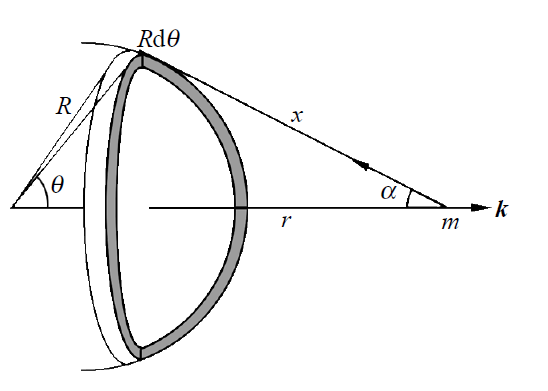
\includegraphics[width=5cm]{Gravitation_1}
	\caption{Gravitational Particle}
	\label{gravitation1}
\end{figure}

 $$d\tau = Rd\theta\,t\,2\pi R\sin\theta \text{ ($t$: width)}$$
 $$\rho = \frac{m'}{4\pi R^2 t}$$
 
 Therefore we have integral:
 \begin{align}
 	F &= \int^{m'}_0 \frac{Gm}{r^2}\,dm\\
 	&=Gm\int^V_0 \frac{\rho}{r^2}\,d\tau\\
 	&=Gm\int^{2\pi}_0 \dfrac{m' t 2\pi R\sin\theta}{4\pi R^2 t x^2}\cos\alpha\,Rd\theta\\
 	&=\frac{1}{2}Gm'm\int^{2\pi}_0 \frac{\sin\theta\cos\alpha}{x^2}\,d\theta
 \end{align}
And we have geometrey relations:
\begin{align}
\left\{
\begin{aligned}
&x^2 = R^2 + r^2 - 2Rr\cos\theta\\
&x\cos\alpha = r - R\cos\theta\\
\end{aligned} 
\right.\\
\left\{
\begin{aligned}
&x\,dx = Rr\sin\theta\,d\theta\\
&\cos\theta = \frac{R^2+r^2-x^2}{2Rr}\\
&x\cos\alpha = r - 2R\cos\theta
\end{aligned} 
\right.
\end{align}
Therefore:
\begin{align}
	F &= \frac{1}{2}Gm'm\int^{r+R}_{\left|r-R\right|} \frac{\cos\alpha}{Rrx}\,dx\\
	&= \frac{1}{2}Gm'm\int^{r+R}_{\left|r-R\right|} \frac{r - 2R\cos\theta}{Rrx^2}\,dx\\
	&=\frac{1}{2}Gm'm\int^{r+R}_{\left|r-R\right|} \frac{1}{Rrx^3}\left(r - \frac{R^2+r^2-x^2}{2r}\right)\,xdx\\
	&=\frac{1}{2}\frac{Gm'm}{Rr}\int^{r+R}_{\left|r-R\right|} \frac{r^2-R^2+x^2}{2r}\,\frac{dx}{x^2}
	\end{align}
	Take the integral:
	\begin{align}
	=\frac{1}{4}Gm'm\frac{r^2-R^2}{Rr^2}\int^{r+R}_{\left|r-R\right|} \frac{dx}{x^2} &+ \frac{1}{4}\frac{Gm'm}{Rr^2}\int^{r+R}_{\left|r-R\right|}\,dx\\
	=-\frac{1}{4}Gm'm\frac{r^2-R^2}{Rr^2}
	\left(\frac{1}{r+R}-\frac{1}{\left|r-R\right|}\right) &+ 
	\frac{1}{4}\frac{Gm'm}{Rr^2}
	\left((r+R)-\left|r-R\right|\right)
\end{align}
Therefore we discuss 2 cases for outside particle $r>R$ and  inside particle $r<R$ separately. With some simple algebra from here:

~\\
For outside particle $r>R$:
\begin{align}
	=-\frac{1}{4}Gm'm\frac{r^2-R^2}{Rr^2}
	\left(\frac{1}{r+R}-\frac{1}{r-R}\right) &+ 
	\frac{1}{4}\frac{Gm'm}{Rr^2}
	\left((r+R)-(r-R)\right)\\
	=-\frac{1}{4}Gm'm\frac{r^2-R^2}{Rr^2}
	\left(\frac{-2R}{r^2-R^2}\right) &+ 
	\frac{1}{4}\frac{Gm'm}{Rr^2}
	\left(2R\right)\\
	=\frac{1}{2}\frac{Gm'm}{r^2} &+ 
	\frac{1}{2}\frac{Gm'm}{r^2}\\
	&= G\frac{m'm}{r^2}
\end{align}
For inside particle $r>R$:
\begin{align}
=-\frac{1}{4}Gm'm\frac{r^2-R^2}{Rr^2}
\left(\frac{1}{r+R}+\frac{1}{r-R}\right) &+ 
\frac{1}{4}\frac{Gm'm}{Rr^2}
\left((r+R)+(r-R)\right)\\
=-\frac{1}{4}Gm'm\frac{r^2-R^2}{Rr^2}
\left(\frac{2r}{r^2-R^2}\right) &+ 
\frac{1}{4}\frac{Gm'm}{Rr^2}
\left(2r\right)\\
=-\frac{1}{2}\frac{Gm'm}{Rr} &+ 
\frac{1}{2}\frac{Gm'm}{Rr}=0
\end{align}
Finally we have:
\begin{align}
	\textbf{F}=\left\{
	\begin{aligned}
	&r>R,-G\frac{m'm}{r^2}\textbf{k}\\
	&r<R,0
	\end{aligned}
	\right.
\end{align}
Regarding a uniform sphere as layers of spherical shells, we can also derive the equation for a uniform sphere (i.e. a celestial object):
\begin{align}
	\textbf{F}=\left\{
	\begin{aligned}
	&r>R,-G\frac{m'm}{r^2}\textbf{k}\\
	&r<R,-G\frac{(r^3/R^3)m'm}{r^2}\textbf{k}=-G\frac{m'm}{R^2}r\textbf{k}
	\end{aligned}
	\right.
\end{align}

Such simple and elegant result is to say, first, the Gravitational force (field) outside of a sphere or spherical shell is equivalent to which of a particle located at its center, taking account of the shape and size of the subject, as a result of integral. No approximation involved. This explains why we can regard earth as a particle even though we are on it and it's shape cannot be ignored. Second, a particle inside a uniform hollow spherical shell is completely weightless, which can be used in many calculations.

Moreover, the result hold true for any force act under inverse square law (i.e. Coulomb's force).









\section{Gravitational Energy}
Derive $U$ for gravitational energy.


\section{Kepler Problem*}
Given $F=-G\dfrac{m'm}{r^3}\textbf{r}$, find the orbit. (General question: find the orbit for a given force law)

\subsection{Using COM Frame}
For two particles in the orbit:
\begin{figure}[H]
	\centering
	\includegraphics{"Kepler Problem"}
	\caption{Kepler Problem}
	\label{Kepler problem}
\end{figure}
\begin{align}
	\left\{
	\begin{aligned}
	&m_1\ddot{\textbf{r}}_1 = -f(r)\textbf{r}\\
	&m_2\ddot{\textbf{r}}_2 = f(r)\textbf{r}
	\end{aligned}
	\right.
\end{align}
	Plus and minus the above equations, we have two equations below:
\begin{align}
	\left\{
	\begin{aligned}
	&m_1\ddot{\textbf{r}}_1 + m_2 \ddot{\textbf{r}}_2 =0\\
	&\ddot{\textbf{r}}_1 - \ddot{\textbf{r}}_2 = -\left(\frac{1}{m_1}+\frac{1}{m_2}\right)f(r)\textbf{r}
	\end{aligned}
	\right.
\end{align}
	For COM:
\begin{align}
	\left\{
	\begin{aligned}
	&m_1 + m_2 = m_C\\
	&m_1\textbf{r}_1 + m_2\textbf{r}_2 = m_C\textbf{r}_C\\
	&\frac{1}{m_1}+\frac{1}{m_2} = \frac{1}{\mu}
	\end{aligned}
	\right.
\end{align}
	Combining (9.2) \& (9.3), we have:
\begin{align}
		\ddot{\textbf{r}}_C &= 0 \text{ (The acceleration of COM is 0)}\\
		\mu \ddot{\textbf{r}} &= - f(r)\textbf{r} \text{ (The problem is equivalent to )}
\end{align}

\subsection{Conservation of Angular Momentum}
\begin{align}
	\bm{M} = \bm{r} \times f(r)\bm{r} = 0
\end{align}
Therefore:
\begin{align}
	\bm{L} &= \bm{r} \times \bm{p} = \bm{C}\\
	&= r\bm{e}_r \times \mu(\dot{r}\bm{e}_r + r\dot{\theta}\bm{e}_\theta) \\
	&= \mu r^2 \dot{\theta} \bm{k}
\end{align}

\subsection{Obtaining the Conservation of Energy: The First Integral}
	Write (9.5) in its component form:
	\begin{align}
	\left\{
		\begin{aligned}
		&\mu(\ddot{r} - r \dot{\theta}^2) = -f(r)\\
		&\mu(r \ddot{\theta} + 2\dot{r}\dot{\theta}) = 0
		\end{aligned}
	\right.
	\end{align}
	
	Integrating the first equation:
	\begin{align}
	\mu(\ddot{r}dr - r \dot{\theta}^2dr) &= -f(r)\\
	\mu \left( \frac{d\dot{r}}{dt} \frac{dr}{dt} dt - r\left(\frac{L}{\mu r^2}\right)^2dr \right)&= -f(r)dr\\
	\mu\dot{r}d\dot{r} - \frac{L^2}{\mu r^3}dr&= -dU\\
	d(\mu\frac{1}{2}\dot{r}^2) + d\left(\frac{L^2}{2\mu r^2}\right)&= G\frac{m'm}{r}\\
	\int d(\mu\frac{1}{2}\dot{r}^2) + \int d\left(\frac{L^2}{2\mu r^2}\right)&= \int d\left(\frac{k}{r}\right)\\
	\mu\frac{1}{2}\dot{r}^2 + \frac{L^2}{2\mu r^2} &= \frac{k}{r}\\
	\frac{1}{2}\mu(\dot{r}^2 + r^2\dot{\theta}^2) &= \frac{k}{r}\\
	\frac{1}{2}\mu(v^2 + (\omega r)^2) - \frac{k}{r} &= E
	\end{align}
	
	Where constant E is the result of indefinite integral, $k \equiv Gm'm$ in this case for the simplicity, represents different force in different cases (e.g. $k_c \equiv kq'q$ for Coulomb force). From the first integral, we derive actually conservation of energy here.

\subsection{The Potential Energy*}
\textbf{Notice:} The following equation is extremely important in solving Kepler problems \textbf{for all force laws} with $U(r)$ representing the integrated potential energy of the force. For inverse square root law, $U(r)=-\dfrac{k}{r}$.
\begin{align}
E &= \frac{1}{2}\mu\dot{r}^2 + \frac{L^2}{2\mu r^2} + U(r) = \text{Constant}\\
U_{\text{eff}}(r) &\equiv \frac{L^2}{2\mu r^2} + U(r) = E-\frac{1}{2}\mu\dot{r}^2
\end{align}	

	\begin{figure}[H]
		\centering
		\includegraphics[width=0.3\linewidth]{"Effective Potential Energy"}
		\caption{Effective Energy Diagram to Determine the Orbit}
		\label{fig:effective-potential-energy}
	\end{figure}
	
\subsection{To Obtain the Orbit: The Second Integral}

The final equation we want is $r(t)$, so to make $\theta$ the only variable, we write the 2 equation:
\begin{align}
	\dot{r} &= \frac{dr}{d\theta}\frac{d\theta}{dt} = \frac{L}{\mu r^2} \frac{dr}{d\theta}\\
	E &= \frac{1}{2}\mu\dot{r}^2 + \frac{L^2}{2\mu r^2} - \frac{k}{r}
\end{align}

Then we take second integral of:
\begin{align}
	\int d\theta &= \int \frac{L}{\mu r^2 \dot{r}}dr\\
	&= \int \dfrac{L}{\mu r^2 \sqrt{\dfrac{2}{\mu}\left(E - \dfrac{L^2}{2\mu r^2} + \dfrac{k}{r}\right)}}dr\\
	&= \int \dfrac{L}{\mu r^2 \sqrt{\dfrac{1}{\mu^2}\left(2\mu E - \dfrac{L^2}{r^2} + 2\mu\dfrac{k}{r}\right)}}dr\\
	&= -\int \dfrac{L}{\sqrt{\left(2\mu E - \dfrac{L^2}{r^2} + 2\mu\dfrac{k}{r}\right)}}d\left(\dfrac{1}{r}\right)\\
	&= -\int \dfrac{L}{\sqrt{2\mu E + \dfrac{\mu^2 k^2}{L^2}-\left( \dfrac{L^2}{r^2} - 2\mu\dfrac{k}{r} + \dfrac{\mu^2 k^2}{L^2} \right)}} d\left(\dfrac{1}{r}\right)\\
	&= -\int \dfrac{1}{\sqrt{2\mu E + \dfrac{\mu^2 k^2}{L^2}-\left(\dfrac{L}{r} - \dfrac{\mu k}{L}\right)^2}} d\left(\dfrac{L}{r} - \dfrac{\mu k}{L}\right)
\end{align}

It seems that we can take the model of $\displaystyle{d\arccos\left(\frac{x}{a}\right) = \int -\dfrac{dx}{\sqrt{a^2 - x^2}}}$:
\begin{align}
\theta &= \arccos\dfrac{\dfrac{L}{r} - \dfrac{\mu k}{L}}{\sqrt{2\mu E + \dfrac{\mu^2 k^2}{L^2}}} + \theta_0\\
\cos(\theta - \theta_0) &= \arccos\dfrac{\dfrac{L}{r} - \dfrac{\mu k}{L}}{\sqrt{2\mu E + \dfrac{\mu^2 k^2}{L^2}}}\\
&= \arccos\dfrac{\dfrac{1}{r}\dfrac{L^2}{\mu k} - 1}{\sqrt{2\mu E\dfrac{L^2}{\mu^2 k^2} + 1}}\\
&= \arccos\dfrac{\dfrac{p}{r} - 1}{\sqrt{E\dfrac{2p}{k} + 1}}\\
&= \arccos\dfrac{\dfrac{p}{r} - 1}{e}\\
\end{align}	

Where:
\begin{align}
	\left\{
	\begin{aligned}
	p &= \dfrac{L^2}{\mu k}\\
	E &= -(1 - e^2)\frac{k}{2p}
	\end{aligned}
	\right.
\end{align}

Therefore:
\begin{align}
	r = \dfrac{p}{1 + e\cos(\theta - \theta_0)}
\end{align}

\begin{center}
	\begin{tabular}{|c|c|c|}
		\hline
		Eccentricity & Energy & Orbit \\
		\hline
		$e = 0$ & $E = -\dfrac{k}{2p}$ & \textsc{Circle} \\
		\hline $0<e<1$
		& $-\dfrac{k}{2p} < E < -\dfrac{k}{2a} < 0$ & \textsc{Ellipse} \\
		\hline $e=1$
		& $E = 0$ & \textsc{Parabola} \\
		\hline $e>1$
		& $E > 0$ & \textsc{Hyperbola} \\
		\hline
	\end{tabular}
\end{center}

\subsection{Another Solution: Binet Equation}

Binet equation:
\begin{align}
	\dfrac{d^2u}{d\theta^2} + u = \dfrac{\mu}{L^2}\dfrac{1}{u^2}F\left(\dfrac{1}{u}\right)
\end{align}

Where: $u = \dfrac{1}{r}$, $F\left(\dfrac{1}{u}\right) = F(r)$.

%-----------------------------------------------------------
%-----------------------------------------------------------

\section{Simple Harmonic Oscillations}

\subsection{General Solution}
Derive the genral solution of SHO.

Write the equation of motion:
\begin{align}
	-kx &= m\ddot{x}
\end{align}
or
\begin{align}
	\ddot{x} + \omega_0^2 &= x,\quad\omega_0^2 = \dfrac{k}{m}
\end{align}

Solve:

\begin{align}
	\left\{\begin{aligned}
	x &= A\cos(\omega t + \phi)\\
	A &= \left(x_0^2 + \dfrac{\dot{x}^2}{\omega_0^2}\right)^{1/2}\\
	\phi &= \arctan \left(-\dfrac{\dot{x}_0}{\omega x_0}\right)\\
	\omega_0 &= \sqrt{\dfrac{k}{m}}
	\end{aligned}\right.
\end{align}

Neither in book nor in class did they mention the derivation. Maybe doesn't matter. 

\subsection{Simple Pendulum}

With Newton's second law, show that: $ \displaystyle{T = 2\pi \sqrt{\frac{L}{g}}} $.

Sol:

The scenario is demonstrated as below:

\begin{figure}[H]
	\centering
	\includegraphics[width=2cm]{"Simple Pendulum"}
	\caption{Simple Pendulum}
	\label{simple-pendulum}
\end{figure}

Therefore:

\begin{align}
\bm{e_\theta}: -mg \sin\theta &= mL \ddot{\theta}\\
\bm{e_\rho}: mg\cos\theta - F_T &= mL\dot{\theta}^2
\end{align}

Assume the solution is $ \theta = A\cos(\omega t + \phi) $;

Set initial condition: $ \theta(t=0)=\theta_0 $, $ \dot{\theta}(t=0)=0 $; Therefore:

\begin{align}
\frac{d\theta}{dt} = \dot{\theta} = -A\omega \sin(\omega t + \phi)=0
\end{align}

That is to say: $ \phi = 0 $. Therefore:

\begin{align}
\theta &= \theta_0 \cos(\omega t)\\
\dot{\theta} &= -\omega \theta_0 \sin(\omega t)\\
\ddot{\theta} &= -\omega^2 \theta_0 \cos(\omega t)
\end{align}

Combined with (2.1), we can find $\omega$:

\begin{align}
-mg \theta_0 \sin(\omega t) &= mL \ddot{\theta} = - mL\omega^2 \theta_0 \cos(\omega t)\\
\omega &= \sqrt{\frac{g}{L}}
\end{align}

Than we can easily find $ T $:

\begin{align}
\omega T &= 2\pi\\
T &= 2\pi\sqrt{\frac{L}{g}}
\end{align}

\section{Wave Equation}

Derive wave equation with dynamics method.

\subsection{Transverse Wave on a Flexible String}
\begin{figure}[H]
	\centering
	\includegraphics[width=0.5\linewidth]{"Displacement in transversive wave"}
	\caption{Displacement in transverse wave}
	\label{fig:displacement-in-transverse-wave}
\end{figure}

Write the equations of motion:
\begin{align}
	&F_{T1}\cos \alpha_1 - F_{T2}\cos \alpha_2 = 0\\
	&F_{T1}\sin \alpha_1 - F_{T2}\sin \alpha_2 = (\rho\,ds)\dfrac{\D^2u}{\D t^2}\label{eq:wave1}
\end{align}

Take approximation for small oscillation of the segment:
\begin{align}
	\cos\alpha_1 \approx \cos\alpha_2 \approx 1, \quad \sin\alpha \approx \tan\alpha \approx \dfrac{\D u}{\D x}, \\ 
	ds = \sqrt{dx^2 + du^2} = dx\sqrt{1+\left(\dfrac{\D u}{\D x}\right)^2} \approx dx
\end{align}

Therefore \ref{eq:wave1} can be written as
	$$F_{T1} = F_{T2} \equiv F_{T}$$
\begin{align}
	F_{T}\left.\dfrac{\D u}{\D x}\right|_{x+dx} - \left.F_{T}\dfrac{\D u}{\D x}\right|_{x} &= (\rho\,dx)\dfrac{\D^2u}{\D t^2}\\
	\left.\dfrac{\D u}{\D x}\right|_{x+dx} = \left.\dfrac{\D u}{\D x}\right|_{x} &+ dx\dfrac{\D^2u}{\D x^2} + \cdots\quad\text{(Taylor Expansion)}\\
	dx\dfrac{\D^2u}{\D x^2} &= \dfrac{\rho\,dx}{F_T}\dfrac{\D^2u}{\D t^2}
\end{align}

With \ref{eq:wave1}
\begin{align}
	\dfrac{\D^2 u}{\D x^2} - \dfrac{1}{v^2}\dfrac{\D^2u}{\D t^2} = 0,\quad v = \sqrt{\dfrac{F_T}{\rho}}
\end{align}

\paragraph{Discussion}
The only factors affects transverse wave speed on flexible string is linear density and tension(which depend both on the outside force and the state of the string, e.g. in non-inertial frame). The higher the force applied or lower the linear density (of the string), the higher the wave speed is. 
\subsection{Longitudinal Wave in a Rubber Band or Air Column}
\begin{figure}[H]
	\centering
	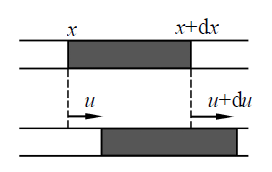
\includegraphics[width=0.4\linewidth]{Longitudinal}
	\caption{Longitudinal wave (The displacement is $du$)}
	\label{fig:longitudinal}
\end{figure}

The equation of motion is
\begin{align}
	\left(\rho_0\,dx\cot S\right)\dfrac{\D^2 u}{\D t^2} = F \label{eq:wave2}
\end{align}

For small stretch or compress $ \Delta L $
\begin{align}
	\displaystyle{\Delta F_T = YS\dfrac{\Delta L}{L}}\\
	Y = \dfrac{L}{S}\left(\dfrac{\D F_T}{\D L}\right)
\end{align} 
\paragraph{Note: Yang's Modulus} Yang's modulus describes tensile elasticity along a line when opposing forces are applied, similar to the role of Hooke's constant in Hooke's law.\\
Then
\begin{align}
	F = \left.YS\dfrac{\D u}{\D x}\right|_{x+dx} - \left.YS\dfrac{\D u}{\D x}\right|_{x} \xlongequal{dx\rightarrow 0} YS\dfrac{\D^2 u}{\D x^2}
\end{align}

Combine with \ref{eq:wave2}
\begin{align}
	\left(\rho_0\,dx\cot S\right)\dfrac{\D^2 u}{\D t^2} &= YS\dfrac{\D^2 u}{\D x^2}\\
	\dfrac{\D^2 u}{\D x^2}-&\dfrac{1}{c^2}\dfrac{\D^2 u}{\D t^2} = 0,\quad \left(c = \sqrt{\dfrac{Y}{\rho_0}}\right)
\end{align}

Note that in the case of gas medium:
\begin{align}
	F_T &\longrightarrow -pS\\
	Y = \dfrac{L}{S}\left(\dfrac{\D F_T}{\D L}\right) &\longrightarrow -\dfrac{L}{S}\left(\dfrac{\D pS}{\D L}\right) = -V\left(\dfrac{\D p}{\D V}\right)_T \equiv B = \dfrac{1}{\kappa_T}
\end{align}

Where B is a proportional coefficient: $p = p_0 + \Delta p,\quad \Delta p = -B\dfrac{\Delta V}{V}$

Then the sound (wave) speed is:
\begin{align}
	v = \sqrt{\dfrac{B}{\rho_0}}
\end{align}

\paragraph{Discussion}
Width is necessary for longitudinal waves, but not for transverse. 

%---------------------------------------
%---------------------------------------


\end{document}

